% 2013 全国卷Ⅰ理科第 6 题：球置于透明无盖正方体容器口，虚线为隐藏棱和被遮挡圆弧。
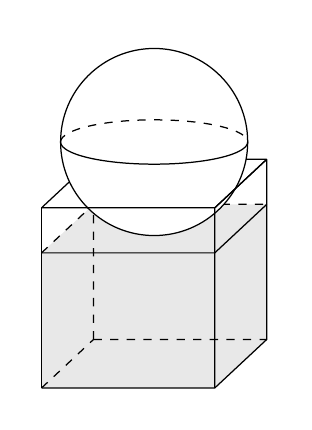
\begin{tikzpicture}[line width=0.45pt, scale=0.88]
  \coordinate (A) at (0,0); \coordinate (B) at (2.5,0);
  \coordinate (C) at (3.25,0.70); \coordinate (D) at (0.75,0.70);
  \coordinate (A') at (0,2.6); \coordinate (B') at (2.5,2.6);
  \coordinate (C') at (3.25,3.3); \coordinate (D') at (0.75,3.3);
  % 水面与容器底面平行，高度为容器高度的 3/4。
  \coordinate (W1) at (0,1.95); \coordinate (W2) at (2.5,1.95);
  \coordinate (W3) at (3.25,2.65); \coordinate (W4) at (0.75,2.65);
  \fill[gray!18] (A)--(B)--(C)--(W3)--(W4)--(W1)--cycle;
  \fill[white] (1.625,3.55) circle (1.35);
  \draw (A)--(B)--(C)--(C');
  \draw (A)--(A');
  \draw (B)--(B')--(C');
  \draw (A')--(B')--(C');
  \draw[dashed] (A)--(D) (D)--(C);
  \draw (W1)--(W2)--(W3);
  \begin{scope}[even odd rule]
    % 容器口后沿仅在球轮廓外显示，前沿仍按透明容器绘制。
    \clip (-0.2,-0.2) rectangle (3.5,5.2)
      (1.625,3.55) circle (1.35);
    \draw (C')--(D')--(A');
    \draw[dashed] (D)--(D') (W1)--(W4)--(W3);
  \end{scope}
  \draw (1.625,3.55) circle (1.35);
  \draw (0.275,3.55) arc[start angle=180,end angle=360,x radius=1.35,y radius=0.32];
  \draw[dashed] (0.275,3.55) arc[start angle=180,end angle=0,x radius=1.35,y radius=0.32];
\end{tikzpicture}
